\section{Collector}
The \textit{Collector} is the main component of our system. The Collector performs different activities: it collects the data form both MQTT and CoAP sensors; it communicates with the devices in order to perform actions; and it stores all the data collected in \textit{MySQL} in the way they can be visualized through \textbf{Grafana} as indicated in the "Database And Data Visualization" paragraph.

In this chapter, all the subcomponents of the Collector will be explained, which are:  MQTT side, CoAP side, DB connection, Data Visualization, and Automation Irrigation System.

\subsection{Command Line Interface}
The \textit{Collector} exposes a \textbf{Command Line Interface}, through which the user can interact with the system. The commands are printed on the terminal when the application starts and they are the following (otherwise indicated the commands are related to CoAP node):

\begin{itemize}
	\item \textit{getDevicesList}: show list of all available sensors (both CoAP and MQTT).
	\item \textit{getTemp}: get the last temperature registered.
	\item \textit{setTemp $<l/u> <value>$}: set desired temperature for specified bound (l for lower, u for upper). Value is an integer expressed in Celsius/Fahrenheit.
	\item \textit{setUnit $<F/C>$}: change temperature measure unit in C (Celsius) or F (Fahrenheit).
	\item \textit{getWeather}: get if the rain sensor feels rain or not.
	\item \textit{getSoilTension}: get the last soil tension registered.
	\item \textit{setSoilTension $<l/u> <value>$}: set desired tension for specified bound (l for lower, u for upper).
	\item \textit{getTapInterval}: get the interval which the tap operates.
	\item \textit{getTapIntensity}: get the intensity which the tap operates.
	\item \textit{setTapInterval $<seconds>$}: set the interval which the tap operates in seconds (acts also on MQTT nodes).
	\item \textit{setTapIntensity $<value>$}: set the intensity which the tap operates (values is a double).
	\item \textit{getWaterLevels}: print the water levels of aquifer and reservoir (MQTT network related).
	\item \textit{start}: start the automatic irrigation system (Java Thread).
	\item \textit{stop}: stop the automatic irrigation system (Java Thread).
	\item \textit{help}: print the commands list.
	\item \textit{quit}: quit the program.
\end{itemize}




\subsection{MQTT Side}
The Collector works as MQTT client: its role consist on receiving periodic measurements about the water levels and make them available to user commands. It is also in charge of sending commands to the reservoir actuator. This mechanism is implemented through the publish/subscribe model: once the Collector is connected with the MQTT broker (Mosquitto process running on user@iot.dii.unipi.it), it starts publishing commands and receiving the updated measurements.
In order to enhance the modularity, 2 separate classes handle respectively the communication with the aquifer and  with the reservoir, according to topics specified above. Collected measurements are stored into a $<nodeId, value>$ Hashmap, and the actual level is taken as the mean of the levels.

The system can potentially handle any number of MQTT devices.



\subsection{CoAP Side}
The Collector plays the roles of both CoAP client and CoAP server. As far as server functionality is concerned, the Collector has a class (called RegistrationServer, which extends CoapServer) which has the task of allowing CoAP nodes to register for the service. In this way, the Collector can use the registered devices acting as a client in order to obtain the data generated by them and also perform actions as indicated in the "Command Line Interface" paragraph and in the "CoAP Network" chapter.

To ensure greater modularity to the code, it was decided to implement dedicated classes for each device, the implementation details are left out here. What is important to underline, however, is the number of devices that can be registered in the system: we thought that in our environment it is possible to insert one or more temperature sensors, one or more soil sensors, a rain sensor and a single tap actuator. The Collector is able to scale autonomously as the temperature and soil sensors number increase thanks to the use of a \textit{List of CoapClient} objects assigned for each resource exposed by the sensors.


\subsection{Database And Data Visualization}
Since we need to save the data obtained, we have implemented a class called \textit{IrrigationSystemDbManager} dedicated to communicating with MySQL to store the data obtained from the devices every time they change. In fact, each device as indicated in the "CoAP Network" chapter has an observable resource, which generate get requests that are captured by our Collector that will call a dedicated function in the \textit{IrrigationSystemDbManager} class to store the data properly.

The data that are saved in the DB are the following (here the sql code to generate the tables):

\begin{verbatim}
CREATE TABLE IF NOT EXISTS `iot_irrigation_system`.`rain` (
  `idrain` INT NOT NULL AUTO_INCREMENT,
  `timestamp` TIMESTAMP NOT NULL DEFAULT CURRENT_TIMESTAMP,
  `isRaining` TINYINT NOT NULL,
  PRIMARY KEY (`idrain`))
ENGINE = InnoDB;


CREATE TABLE IF NOT EXISTS `iot_irrigation_system`.`soilMoisture` (
  `idsoilMoisture` INT NOT NULL AUTO_INCREMENT,
  `timestamp` TIMESTAMP NOT NULL DEFAULT CURRENT_TIMESTAMP,
  `soilValue` DOUBLE NOT NULL,
  PRIMARY KEY (`idsoilMoisture`))
ENGINE = InnoDB;


CREATE TABLE IF NOT EXISTS `iot_irrigation_system`.`tap` (
  `idtap` INT NOT NULL AUTO_INCREMENT,
  `timestamp` TIMESTAMP NOT NULL DEFAULT CURRENT_TIMESTAMP,
  `intensity` DOUBLE NOT NULL,
  `interval` INT NOT NULL,
  PRIMARY KEY (`idtap`))
ENGINE = InnoDB;


CREATE TABLE IF NOT EXISTS `iot_irrigation_system`.`temperature` (
  `idtemperature` INT NOT NULL AUTO_INCREMENT,
  `timestamp` TIMESTAMP NOT NULL DEFAULT CURRENT_TIMESTAMP,
  `tempValue` TINYINT(1) NOT NULL,
  PRIMARY KEY (`idtemperature`))
ENGINE = InnoDB;


CREATE TABLE IF NOT EXISTS `iot_irrigation_system`.`waterLevelAquifer` (
  `idwaterLevel` INT NOT NULL AUTO_INCREMENT,
  `timestamp` TIMESTAMP NOT NULL DEFAULT CURRENT_TIMESTAMP,
  `nodeId` VARCHAR(10) NOT NULL,
  `waterLevel` DOUBLE NOT NULL,
  PRIMARY KEY (`idwaterLevel`))
ENGINE = InnoDB;


CREATE TABLE IF NOT EXISTS `iot_irrigation_system`.`waterLevelReservoir` (
  `idwaterLevel` INT NOT NULL AUTO_INCREMENT,
  `timestamp` TIMESTAMP NOT NULL DEFAULT CURRENT_TIMESTAMP,
  `nodeId` VARCHAR(10) NOT NULL,
  `waterLevel` DOUBLE NOT NULL,
  PRIMARY KEY (`idwaterLevel`))
ENGINE = InnoDB
\end{verbatim}


Talking about \textbf{Data Visualization} we used \textit{Grafana} for displaying most of the information presented above\footnote{We didn't plot the tap interval, since it can be obtained by subtracting two adjacent point in the tap intensity graph.}. An example of what we plot is shown in the following figure:

\begin{figure}[H]
	\begin{subfigure}{\textwidth}
	\centering
		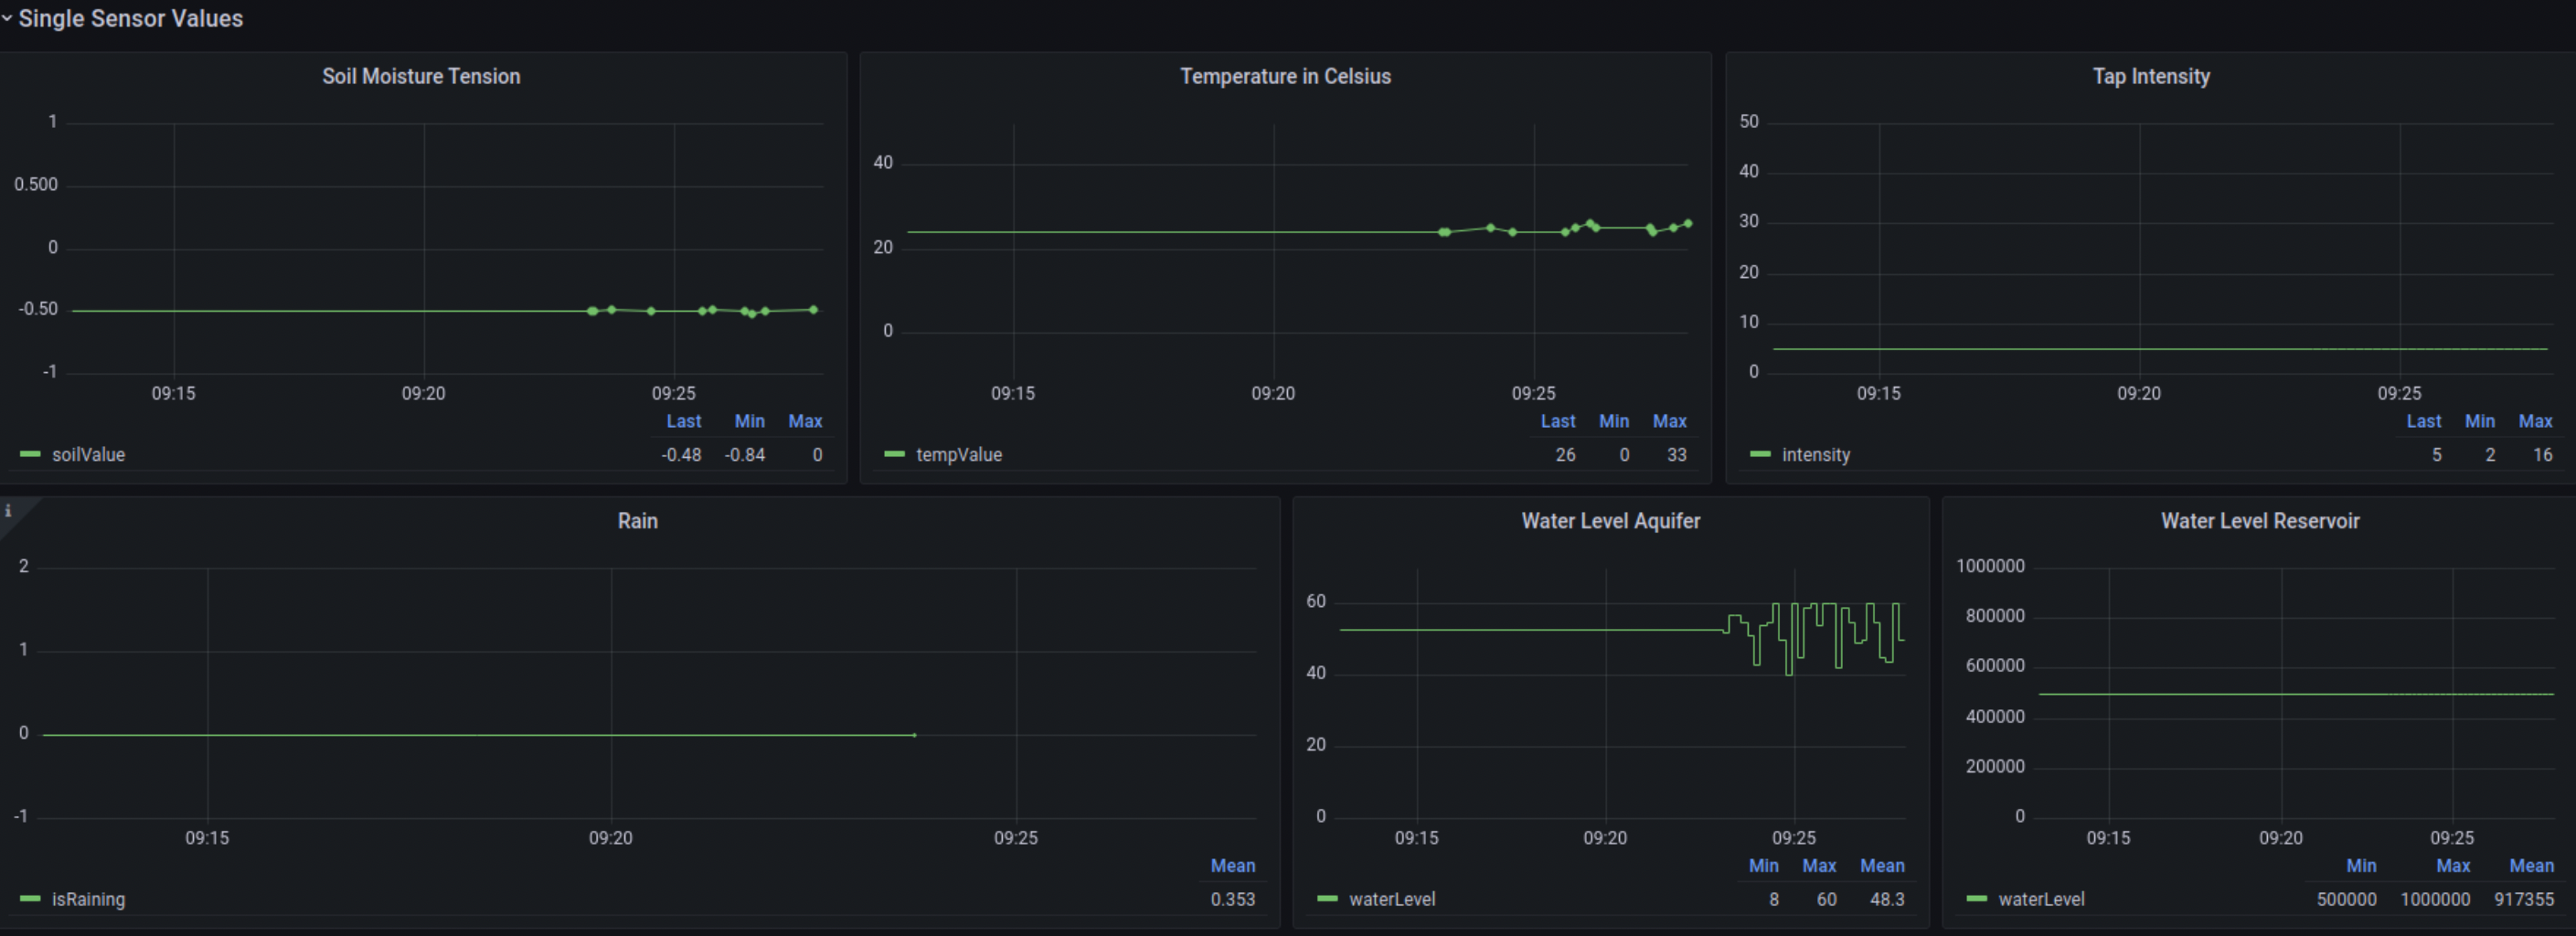
\includegraphics[width=.83\linewidth]{img/grafana.png} 
	\end{subfigure}
\end{figure}

\subsection{Automatic Irrigation System}
The Automatic Irrigation System is the hearth of the proposed solution: it is in charge of periodically computing the water need based on data reported by the CoAP sensors and selecting the water source based on the measurements of the MQTT devices. The Automatic Irrigation System is a parallel Java Thread that can be started or stopped at any time by the user. At every iteration the system:
\begin{itemize}
	\item Collects into a Parameters object all the retrieved data needed to estimate the water need
	\item Computes the need based on the following formula: 

\begin{lstlisting}
if(p.isRaining){
  Logger.log("[Irrigation System]: It's Raining, no irrigation is needed");
  continue;
}

switch(p.soilStatus){
   case TOO_LOW:
       level = Levels.LOW;  //low soil moisture means wet soil, so little water is needed
       break;
   case NORMAL:
       level = Levels.MEDIUM;
       break;
   default:
       level = Levels.HIGH;
}
if (p.temperatureStatus == BoundStatus.TOO_HIGH)
     level = level.increaseLevel();

\end{lstlisting}


	\item Determines the actual tap output, given by \textit{level*tapIntensity}.
	\item Determines the water source, based on the water policy reported in the first paragraph and implemented as follows.

\begin{lstlisting}
if (need>p.aquiferLevel)
    WhereWater=RESERVOIR;
WhereWater=AQUIFER;
\end{lstlisting}	
	
	\item Sends a command to the reservoir to fetch/store water
\begin{lstlisting}
if (source == RESERVOIR){
     rc.changeReservoirLevel(0-quantity);
     Logger.log("\tFetched "+quantity + " from the RESERVOIR");
}
else{
     rc.changeReservoirLevel(p.aquiferLevel-quantity);
     Logger.log("\tFetched "+p.aquiferLevel+"cm^3 from the aquifer");
     Logger.log("\t" + quantity + "cm^3 of them are output of the tap,");
     Logger.log("\t" + (p.aquiferLevel-quantity) + "cm^3 of them are stored in the reservoir");
}
\end{lstlisting}
\end{itemize}

